\scanpage{340}
% R340.01 | text | top, lines 1--12 | Ce calcul suggère fortement
This calculation strongly suggests that the relations \deleted{\unsure{pa|by}} (64) already imply (68)\ldots{} it is \unsure{even} very nearly a proof\ldots{} If we admit this point, it only remains to verify that the preceding conditions \inserted{(64)} (i.e. essentially already (51) to (56) except (55)) also imply (55), i.e. the independence of the $\varepsilon_0,\varepsilon_1$ in every fiber, i.e. that $N_0,N_1$ are non-homothetic in \unsure{every} fiber. Now (67)
% R340.02 | display | upper middle, line 13 | N_1=tilde sigma(N_0)
\[
(*)\qquad N_1=\widetilde\sigma(N_0),\ \unsure{\deleted{\text{and}}}\ \inserted{=\widetilde\rho(\unsure{N_1|N_0})}\ \deleted{N_0=\unsure{\widetilde\sigma(N_1)}}\,\unsure{:}
\]
% R340.03 | text | middle, line 14 | Si on avait sur une fibre
If we had on a fiber
% R340.04 | display | middle, line 15 | N_1=lambda N_0
\[
\unsure{(\deleted{74})}\qquad N_1=\lambda N_0
\]
% R340.05 | text | middle, lines 16--18 | on en conclurait
we would conclude from this, by \unsure{applying} \deleted{$\widetilde\sigma$ and} using $\widetilde\sigma^2=1$, \inserted{and $\widetilde\rho^3=1$,} \inserted{the relations} \deleted{$\widetilde\sigma(N_1)=N_0$, $\widetilde\sigma(N_0)=N_1$}
% R340.06 | display | lower middle, lines 19--20 | N_0=lambda N_1
\[
\deleted{\unsure{(**)}\qquad
\left\{\begin{aligned}
N_0&=\lambda N_1\unsure{\deleted{=\lambda^2}},\quad
\text{thus }\deleted{\lambda^2=1}\ N_0=\lambda^2N_0\quad\text{whence}\\
\lambda^2&=1.
\end{aligned}\right.}
\]
% R340.07 | text | lower middle, line 21 | Mais un calcul immédiat
\deleted{But an immediate calculation also gives}
% R340.08 | display | lower middle, line 22 | N_0=rho^{-1}N
\[
\deleted{(**)\qquad N_0=\rho^{-1}N,\quad N_1\unsure{-}}
\]
% R340.09 | display | lower, line 23 | lambda^2=1,lambda^3=1
\[
\lambda^2=1,\quad\lambda^3=1\qquad\text{whence }\lambda=1
\]
% R340.10 | text | lower, lines 24--28 | i.e. N_0=N_1
i.e. $N_0=N_1$ i.e. $N_0$ commutes with $\sigma,\rho$ thus also $N=-\sigma N_0$ \inserted{$=\rho^{-1}N_0$} commutes with $\sigma,\rho$, and since $N=\sigma+\rho$, $\sigma$ and $\rho$ commute. But then
% R340.11 | text | bottom left | 339
\mspage{339}

\scanpage{341}
% R341.01 | text | top centre | 471
\mspage{471}
% R341.02 | display | top, lines 1--2 | (sigma+rho)^2
\[
(\sigma+\rho)^2=\underbrace{\sigma^2}_{-1}+\underbrace{\rho^2}_{\rho-1}+2\sigma\rho=\rho-2+2\sigma\rho=
\]
% R341.03 | text | upper, line 3 | donc la relation
thus the relation $(\sigma+\rho)^2=\sigma+\rho$ is written
% R341.04 | display | upper, lines 4--5 | rho-2+2 sigma rho
\[
\deleted{\rho}-2+2\sigma\rho=\sigma+\deleted{\rho}\qquad\text{i.e.}
\]
\[
\deleted{\unsure{(**)}}\qquad
2\sigma\rho=\sigma+2\quad\text{that is}\quad
\underbrace{2\sigma^2\rho}_{-2\rho}=\underbrace{\sigma^2}_{-1}+2\sigma
\quad\text{i.e.}\quad 2(\sigma+\rho)=1
\]
% R341.05 | text | upper middle, lines 6--14 | Prenant les traces
\deleted{Taking the traces of both sides, and using $\operatorname{Tr}\sigma\rho=2$ (74), $\operatorname{Tr}\sigma=0$, $\operatorname{Tr}1=2$, we find $4=4$, no contradiction but taking the determinants \inserted{of both sides of \unsure{(**)},} we find (\deleted{\unsure{det}} admitting that $\det\sigma=\det\rho=1$, which is a consequence of (64) provided only that we require in addition that $\sigma,\rho$ be regular i.e. be scalars on no fiber) we find}
% R341.06 | margin note | left of lines 12--14 | double vertical stroke
\margin{$\Vert$}
% R341.07 | display | middle, line 15 | 2^2=2^2+2 Tr sigma
\[
\deleted{(***)\qquad 2^2=2^2+2\underbrace{\operatorname{Tr}\sigma}_{0}+\underbrace{(\det\sigma)^{\unsure{2}}}_{1}\quad\text{i.e.}\quad 1=0}
\]
% R341.08 | text | middle, lines 16--17 | ce qui est absurde
\deleted{which is absurd. whence, taking}

\deleted{I \unsure{it}} i.e.
% R341.09 | display | lower middle, line 18 | 2N=1
\[
(**)\qquad 2N=1,
\]
% R341.10 | text | lower middle, line 19 | d'où, en prenant
whence, taking the determinants
% R341.11 | display | lower middle, line 20 | 4 det N=1
\[
4\underbrace{\det N}_{0}=1\qquad\text{i.e.}\quad 0=1,\quad\text{\uline{absurd}.}
\]
% R341.12 | text | lower, lines 21--25 | Remarque Je ne serais pas étonné
\deleted{I will not be}

\uline{Remark} I would not be surprised if we also had conditions equivalent to (51) to (56) in the form
% R341.13 | display | bottom, line 26 | (75) sigma^2+1
\[
(75)\qquad \sigma^2+1=\rho^{\unsure{3|2}}\unsure{-|+}\rho+1=0,\quad
\varepsilon_0\mathrel{\overset{\mathrm{dfn}}{=}}-\sigma^{-1}\rho\ \text{is regular unipotent}
\]
% R341.14 | text | bottom left | 340
\mspage{340}

\scanpage{342}
% R342.01 | text | top, lines 1--4 | en exigeant de plus
requiring in addition, if need be, that $\sigma,\rho$ also be regular i.e. be scalars on no fiber. One would have to convince oneself that this implies that
% R342.02 | display | upper, line 5 | N=dfn rho+sigma
\[
N\mathrel{\overset{\mathrm{dfn}}{=}}\rho+\sigma
\]
% R342.03 | text | upper, line 6 | satisfait bien la relation
does satisfy the idempotence relation
% R342.04 | display | upper, line 7 | N^2-N=0
\[
(75)\qquad N^2-N=0
\]
% R342.05 | text | upper middle, line 8 | ce qui équivaut
(which is equivalent, if $N$ regular, to
% R342.06 | display | upper middle, line 9 | Tr N=1,det N=0
\[
(77)\qquad \operatorname{Tr}N=1,\quad\det N=0\qquad (?)
\]
% R342.07 | text | middle, lines 10--13 | Mais N est régulier
But $N$ is regular, for if on a fiber \unsure{it were} a scalar we would have that (restricting to this fiber) $\rho$ and $\sigma$ commute, we would have
% R342.08 | display | middle, lines 14--15 | -sigma^{-1}rho=sigma rho
\[
\begin{aligned}
-\sigma^{-1}\rho&=\sigma\rho=\varepsilon_0=1+N_0\\
-\inserted{\unsure{''}}\rho\sigma^{-1}&=\rho\sigma=\varepsilon_1=1+N_1,
\end{aligned}
\]
% R342.09 | deletion | middle, beneath second epsilon identity | Prenant
\deleted{\unsure{Taking} $\unsure{\varepsilon_0=\det\rho}$}

\deleted{with}
% R342.10 | display | middle-lower, lines 16--18 | (1-sigma rho)^2=0
\[
(1-\sigma\rho)^2=0\quad\text{i.e.}\quad
1-2\sigma\rho+\underbrace{\sigma^2}_{-1}\underbrace{\rho^2}_{\rho-1}=0\quad\text{i.e.}
\]
\[
1-2\sigma\rho+1-\rho=0\quad\text{i.e.}\quad 2=\rho+2\sigma\rho
\]
% R342.11 | text | lower, line 19 | soit, en multipliant
that is, multiplying by $\sigma$
% R342.12 | display | lower, line 20 | 2 sigma=rho sigma+2 sigma^2 rho
\[
2\sigma\unsure{=}\rho\sigma+2\underbrace{\sigma^2}_{-1}\rho
\quad\text{i.e.}\quad 2\underbrace{(\sigma+\rho)}_{N}=\rho\sigma
\]
% R342.13 | text | lower, lines 21--23 | Mais par hyp.
But by hypothesis we have $N=\lambda.1$, $\lambda$ a scalar, whence $\rho\sigma=2\lambda$, and taking the determinants
% R342.14 | display | lower, line 24 | det(rho sigma)=4 lambda^2
\[
\det\underbrace{(\rho\sigma)}_{1}=4\lambda^2
\]
% R342.15 | text | bottom, line 25 | i.e. 2 inv.
i.e. $\deleted{\unsure{4}}\ 2$ invertible and $\lambda=\dfrac{\varepsilon}{2}$, with $\varepsilon^2=1$,
% R342.16 | display | bottom, lines 26--27 | rho sigma=epsilon
\[
\begin{aligned}
\text{i.e.}\qquad&\rho\sigma=\varepsilon\qquad\varepsilon^2=1,\\
&\rho^2\underbrace{\sigma^2}_{-1}=1\qquad\underbrace{\rho^2}_{\rho-1}=-1,\quad\text{i.e.}\quad\rho=0,\quad\text{\uline{absurd}}
\end{aligned}
\]
% R342.17 | text | bottom left | 341
\mspage{341}

\scanpage{343}
% R343.01 | text | top centre | 472
\mspage{472}
% R343.02 | deletion | top, line 1 | Mais Tr N=0
\deleted{But $\operatorname{Tr}N=0$ \unsure{by}}
% R343.03 | text | upper, lines 2--4 | Donc N est régulier
Thus $N$ is regular, it remains to prove (77).

But $\operatorname{Tr}N=\underbrace{\operatorname{Tr}\sigma}_{0}+\underbrace{\operatorname{Tr}\rho}_{1}=1$, OK, remains to prove $\det(\rho+\sigma)=0$ but
% R343.04 | display | upper middle, line 5 | det(rho+sigma)
\margin{\figure{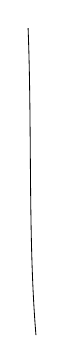
\begin{tikzpicture}[x=1mm,y=1mm]\draw[line width=.3pt] (1,0) .. controls (0,12) and (.5,26) .. (0,39);\end{tikzpicture}}}
\[
\det(\rho+\sigma)=\deleted{\underbrace{\det\rho}_{1}+\underbrace{\det\sigma}_{1}+\operatorname{Tr}(\sigma\rho)}
\]
% R343.05 | deletion | upper middle, lines 5--6 | et la relation équivaut
\deleted{and the relation is equivalent}
% R343.06 | display | middle, lines 6--9 | det sigma(1+sigma^{-1}rho)
\[
\begin{aligned}
\unsure{''}\quad
\det\unsure{(}\unsure{\deleted{\rho}\inserted{\sigma}}(1+\sigma^{-1}\rho)
&=\det\sigma\ \underbrace{\det(1+\sigma^{-1}\rho)}_{\underbrace{\det\sigma^{-1}\rho}_{(\det\sigma)^{-1}\det\rho}+\operatorname{Tr}(\underbrace{\sigma^{-1}\rho}_{-\sigma\rho})+1}\\
&=\overbrace{\det\sigma}^{1}+\overbrace{\det\rho}^{1}+\underbrace{\det\sigma}_{1}\operatorname{Tr}(\sigma^{-1}\rho)
\end{aligned}
\]
% R343.07 | margin note | diagonal left margin, beside lines 7--11 | calcul déjà fait
\margin{calculation already done See page \unsure{--} ? (cf. formula (69))}
% R343.08 | display | middle, line 10 | det(sigma+rho)=2+Tr(sigma^{-1}rho)
\[
\text{i.e.}\qquad\det(\sigma+\rho)=2+\operatorname{Tr}(\sigma^{-1}\rho)=2\unsure{-}\operatorname{Tr}\sigma\rho,\quad\text{thus}
\]
% R343.09 | text | middle, line 11 | la condition det N=0
the condition $\det N=0$ is equivalent to (69)
% R343.10 | display | middle, line 12 | Tr sigma rho=2
\[
\operatorname{Tr}\sigma\rho=2
\]
% R343.11 | text | lower, lines 13--17 | Pour prouver cette relation
To \deleted{\unsure{it}} prove this relation \inserted{(or \unsure{versions|neighboring ones} \unsure{tested|such})}, we can think of \deleted{starting}\inserted{proceeding} as earlier, \unsure{except that I} \unsure{have} started from (68) instead of (75). This is not entirely elucidated -- to return to the attack!
% R343.12 | text | bottom left | 342
\mspage{342}

\scanpage{344}
% R344.01 | text | top centre | 473
\mspage{473}
% R344.02 | text | heading | VII Récapitulation sur les épinglages
$\overline{\text{\uline{VII}}}$\quad \uline{Recapitulation on pinnings.}
% R344.03 | text | upper, lines 2--4 | On désigne par G,SG,PG
\deleted{\unsure{1)}} We denote by $G,SG,PG$ forms of $\mathrm G\ell(2)_S$, $\mathrm S\ell(2)_S$, $\unsure{\mathrm{GP}(1)}_S$ \unsure{associated} to the same Azumaya Algebra $\mathcal M$, i.e. to a bundle of projective lines $\unsure{\mathbb P|\mathcal P}$, over $S$.
% R344.04 | text | subsection heading | Sections régulières de G
1) \uline{Regular sections of} $G$.
% R344.05 | text | upper middle, line 6 | Soit rho une section
Let $\rho$ be a section of $\unsure{\mathcal M}$ \inserted{(not necessarily invertible)}, put
% R344.06 | display | upper middle, line 7 | v=det rho,w=Tr rho
\[
(1)\qquad \unsure{v|\nu}=\det\rho,\quad w=\operatorname{Tr}\rho
\]
% R344.07 | text | upper middle, line 8 | de sorte qu'on aura
so that we have\deleted{ura} the Hamilton-Cayley equation
% R344.08 | display | upper middle, line 9 | rho^2-w rho+v=0
\[
(2)\qquad \rho^2-w\rho+\unsure{v|\nu}=0\qquad\text{i.e.}\quad\rho^2=w\rho-\unsure{v|\nu}
\]
% R344.09 | text | middle, line 10 | Proposition Conditions équivalentes
\uline{Proposition} Equivalent conditions:
% R344.10 | text | middle, line 11 | a) rho n'est un scalaire
a) $\rho$ is not a scalar on any fiber.
% R344.11 | text | middle, lines 12--13 | a') A_rho=O_S+O_S rho
\unsure{a')} $\mathcal A_\rho=\underline{\mathcal O}_S+\underline{\mathcal O}_S\rho$ is a submodule \unsure{locally|locally} a free direct summand of rank $2$ of $\mathcal M$.
% R344.12 | margin note | left, beside conditions a' and b | NB À cause de (2)
\margin{N.B. Because of (2), $\mathcal A_\rho$ is a sub-\uline{Algebra} of $\mathcal M$.}
% R344.13 | text | middle, lines 14--16 | b) Il existe loc. (Zar)
b) (If $\mathcal M=\underline{\operatorname{End}}_{\mathcal O_S}(F)$) There exists locally (Zariski) a section $\unsure{e_0|E_0}$ of $F$ such that $(e_0,\deleted{\unsure{\rho.}}e_1\mathrel{\overset{\mathrm{dfn}}{=}}\rho(e_0))$ form a basis of $F$
% R344.14 | text | middle-lower, lines 17--18 | b') Il existe loc. Zar
b') (If $\mathcal M=\underline{\operatorname{End}}_{\mathcal O_S}(F)$) There exists locally Zariski a ``line subbundle'' $D_0\subset F$, such that
% R344.15 | display | middle-lower, line 19 | F=D_0+D_1
\[
F=D_0+D_1,\quad\text{where }D_1=\rho(D_0)
\]
% R344.16 | text | lower, lines 20--22 | b'') Le O_S[T]-module
\unsure{b'')} (If $\mathcal M=\underline{\operatorname{End}}_{\mathcal O_S}(F)$.) The $\mathcal O_S[T]$-module $F_\rho$ ($\unsure{:}$ $T$ \unsure{is|being} an indeterminate, which operates on $F$ by $\rho$) is \deleted{\unsure{isomorphic} to $\underline{\mathcal O}_S$} \inserted{\deleted{\unsure{locally}} cyclic} locally (Zariski).
% R344.17 | text | lower, lines 23--24 | c) Le O_S[T]-module
c) (If $\mathcal M=\underline{\operatorname{End}}_{\mathcal O_S}(F)$) The $\underline{\mathcal O}_S[T]$-module $F_\rho$ \unsure{is|$\to$} isomorphic to
% R344.18 | display | lower, line 24 | O_S[T]/(T^2-wT+v)
\[
\underline{\mathcal O}_S[T]/(T^2-wT+\unsure{v|\nu})
\]
% R344.19 | text | bottom, lines 25--26 | c') il existe localt Zar une base
c') \inserted{(case $\mathcal M=\underline{\operatorname{End}}(F)$)} $\exists$ \unsure{locally|locally} Zariski a basis $e_0,e_1$ of $F$, such that the matrix of $\rho$ \unsure{with respect|p.v.} to this basis
% R344.20 | text | bottom left | 343
\mspage{343}

\scanpage{345}

is
\[
(3)\qquad \rho_{e_0,e_1}=\begin{pmatrix}0&-\unsure{v|\nu}\\1&w\end{pmatrix}
\]
\margin{(i.e. $\rho e_0=e_1$ whence \deleted{$\rho e_1=$}
$\rho e_1=\unsure{-v\rho e_0-w e_0}$}

c'') \inserted{(Case $\mathcal M=\underline{\operatorname{End}}_{\underline{\mathcal O}_S}(F)$)}
$\exists$ locally Zariski a basis $(e_0,e_1)$ of $F$ such that the matrix of $\rho$ with respect to it is
\[
(4)\qquad \rho_{e_0,e_1}=\begin{pmatrix}0&1\\-v&w\end{pmatrix}
\]

d) The commutant of $\rho$ in $\mathcal M$ is reduced to
$\mathcal A_\rho=\underline{\mathcal O}_S+\underline{\mathcal O}_S\rho$, and it remains so after every base change $S'\to S$.

d') \unsure{Item|Item} in each fiber.

\uline{Proof}\quad $a\Longleftrightarrow a'$ trivial (linear algebra of the Modules $\mathcal M$ and of the submodules $\underline{\mathcal O}_S1$ locally direct summands)

$b\Longleftrightarrow b'\Longleftrightarrow b''$ trivial, $b)\Longrightarrow a)$ as well.

$a\Longrightarrow b$ it suffices to choose $e_0$ \deleted{in}\inserted{on} a \deleted{\unsure{field}}\inserted{fiber} so as not to be an eigenvector under $\rho$ (possible over a field, for a nonscalar operator) then to lift in a neighborhood.

\inserted{$b\Longleftrightarrow$}$c)\Longleftrightarrow c')$ trivial ; \deleted{$c')\Longleftrightarrow c'')$ \unsure{for the}}\inserted{the bases for which}
$\rho_{e_0,e_1}$ is of the form $\begin{pmatrix}0&-v\\1&w\end{pmatrix}$ \unsure{are} precisely the bases of the form $(e_0,e_1=\rho e_0)$.

$c')\Longleftrightarrow c'')$ means that if $\rho$ satisfies the conditions under consideration, ${}^t\rho$ does too. (\deleted{\unsure{therefore}} and conversely it follows from this that the condition for ${}^t\rho$ implies it for $\rho={}^t({}^t\rho)$\deleted{\unsure{$\}$}}, i.e. $c'')\longrightarrow c')$) --- but this is immediate in the form a).

Thus the conditions a) to c'') are equivalent, moreover $d)\Longrightarrow d')\Longrightarrow a)$ is trivial, it remains to prove that $b$ (for example) $\Rightarrow d)$.
\deleted{If $u$ commutes}\inserted{Since $b$ \unsure{stable}} under base change, it suffices to see that

\mspage{344}

\scanpage{346}
\mspage{474}

\deleted{\uline{Corollary 2}}

\uline{N.B.}\quad \unsure{In} fact, $G=\underline{\mathcal M}^{*}$ operates on $\underline{\mathcal M}$ (by inner automorphisms) or on $G$, or $SG$, via $PG=\underline{\mathcal M}^{*}/\mathbb G_m$, and $PG$ is an fppf quotient of $SG$ (and \unsure{even|=} for the topology (étale), if 2 invertible).

So we see that \inserted{in} the preceding conjugation criterion, in the formula
\[
(6)\qquad \rho'=\operatorname{int}(\alpha)\rho=\alpha\rho\alpha^{-1},
\]
\unsure{we may assume} $\alpha\in\Gamma\unsure{\mathrm S\ell(2)|SG}$.

\deleted{\uline{Proposition} Let $\unsure{\varepsilon}$ be}\inserted{\uline{Corollary 2} Let} $\rho,\unsure{\zeta|\xi}$ be two sections of $G$, $\rho$ being regular. For us to be able to find locally Zariski an $\alpha\in\Gamma G$ such that
\[
(7)\qquad [\alpha,\rho]=\zeta\qquad\text{i.e.}\quad \alpha\rho\alpha^{-1}=\zeta\rho
\]
it is necessary and sufficient that we have

a) $\zeta\rho$ is regular, i.e. $\zeta$ \deleted{$\unsure{\neq}$} non-homothetic to $\rho^{-1}$ on any fiber

b) $\det\zeta=1$, $\operatorname{Tr}\zeta\rho=\operatorname{Tr}\rho$

(We can then take $\alpha$ in $SG$\ldots)

\unsure{This is|These are} only the conditions of corollary 1 \deleted{\unsure{of}} for conjugation of $\zeta\rho$ to $\rho$, the condition $\det\zeta\rho=\det\rho$ also being written as $\det\zeta\det\rho=\det\rho$ i.e. $\det\zeta=1$.

\uline{Corollary 3} The indeterminacy of $\alpha$ in the solution of (7) is of the form $\alpha\mapsto\alpha\uline{t}$, with $\uline{t}$ a section of $\underline{\mathcal A}_\rho^*$, i.e. $t=c\rho+d$, with $c,d\in\Gamma\underline{\mathcal O}_S$, $\det(c\rho+d)$ invertible.
\inserted{i.e. $\boxed{\text{\textcircled{8}}\quad c^2\unsure{v|\nu}+wcd\deleted{\text{invertible}}+d^2\quad\text{invertible}}$}
(where, $v=\det\rho$, $w=\operatorname{Tr}\rho$, cf. (1)).

\mspage{345}

\scanpage{347}

if $u$ is a section of $\mathcal M$ \deleted{such that} which commutes with $\rho$, then $u=a+b\rho$ $(a,b\in\Gamma\underline{\mathcal O}_S)$. By a) $a$ and $b$ are unique, and this shows that the question is fppf local. \unsure{We may assume} therefore $\mathcal M=\underline{\operatorname{End}}(F)$, $F$ equipped with a basis $(e_0,e_1=\rho(e_0))$. \deleted{\unsure{and}} We will have, if
\[
\deleted{ue_1=u\rho e_0=\rho=}
\]
\[
u(e_0)=ae_0+be_1\inserted{{}=u'(e_0)}\qquad
\deleted{\text{put }u'=a+b\rho}\inserted{\text{where}}\quad u'=a+b\rho,
\]
\[
\deleted{u(e_1)=u\rho(e_0)=\rho\underline{ue_0}=\rho(ae_0+be_1)=a\rho(e_0)+b\rho(e_1)}
\]
and if $u$ \unsure{commutes} \deleted{$=ae_1+$} with $\rho$, we will have
\[
u(e_1)=u\rho(e_0)=\rho u(e_0)\deleted{{}=\rho(ae_0+}
\]
likewise
\[
u'(e_1)=u'\rho(e_0)=\rho u'(e_0)\qquad\text{for }u'\text{ commutes with }\rho
\]
therefore
\[
u(e_0)\unsure{=|\neq}\unsure{u(e'_0)|u'(e_0)},\quad u(e_1)=u'(e_1)\qquad\text{therefore }u=u',
\]
q.e.d.

\uline{Definition :} A section \inserted{of $\mathcal M$} which satisfies the equivalent conditions of the proposition is called \uline{regular}. \unsure{Item|Item} for sections of $G$, $SG$, interpreted as sections of $\mathcal M$ --- \deleted{they are} such a section is regular iff at no point is it a scalar, i.e. is not in the center. This \unsure{remains|is} stable under multiplication by an invertible scalar --- whence by passage to the quotient we deduce the notion of a regular section of $PG$ --- these are the sections which are not $=1$ on any fiber.

\uline{Corollary 1} Let $\rho,\rho'$ be two \deleted{regular} sections of $\mathcal M$, \inserted{$\rho$ being regular.} For them to be conjugate (locally Zariski) via $\mathcal M^*$, it is necessary and sufficient that \deleted{$\rho$} a) $\rho'$ be regular (Condition \inserted{of regularity} \deleted{\illegible{1}}) and b) we have
\[
(5)\qquad \det\rho=\det\rho',\quad \operatorname{Tr}\rho=\operatorname{Tr}\rho'
\]
(``Numerical condition''

\mspage{346}

\scanpage{348}
\mspage{475}

This follows from the equivalence $a)\Longleftrightarrow d)$ of the proposition.

\uline{Proposition} Let
\[
(9)\qquad \varepsilon=1+N
\]
be a section of $\mathcal M$. Equivalent conditions

\[
\text{a)}\quad (10)\quad
\begin{gathered}
\det\varepsilon=\det1\quad(=1)\\
\operatorname{Tr}\varepsilon=\operatorname{Tr}1\quad(=2)
\end{gathered}
\qquad \deleted{\varepsilon\text{ regular}}\quad\text{and }\varepsilon\text{ regular}
\]
\margin{\uline{N.B.}\quad $\det(1+N)=1+\operatorname{Tr}N+\det N$\quad $\operatorname{Tr}(1+N)=2+\operatorname{Tr}N$.}
\[
\text{b)}\quad (11)\quad \det N=\operatorname{Tr}N=0\qquad\text{and }N\text{ regular}
\]

c) (If $\mathcal M=\underline{\operatorname{End}}_{\underline{\mathcal O}_S}(F)$) $\exists$ line bundle $D\subset F$ such that we have
\[
N(F)=D,\quad N(D)=0
\]
(Then $D$ is uniquely determined by $\varepsilon$ i.e. by $N$, \deleted{and conversely} \inserted{$D$ determines $N$ modulo homothety})

\inserted{c') (If $\mathcal M=\underline{\operatorname{End}}_{\underline{\mathcal O}_S}(F)$). $\exists$ locally \unsure{basis|Zariski} $e_0,e_1$ such that $\varepsilon=\begin{pmatrix}1&1\\0&1\end{pmatrix}$ i.e. $N=\begin{pmatrix}0&1\\0&0\end{pmatrix}$}

d) $\exists$ Borel $B\subset G$, such that $\varepsilon$ is a section everywhere $\ne1$ of $B_u$.

d') \deleted{\unsure{If}}$\exists$ Borel $SB\subset SG$, such that $\varepsilon$ is a section everywhere $\ne1$ of $(SB)_u$.

\deleted{\unsure{Proof}} Moreover, $D,B,SB$ are well determined by $\varepsilon$ i.e. by $N$, and determine $N$ up to homothety.

\uline{Definition :} we \deleted{say} \unsure{that} $\varepsilon$ is (strictly) unipotent iff we have $\det\varepsilon=1$, $\operatorname{Tr}\varepsilon=2$, that $N$ is \uline{strictly nilpotent} \unsure{iff|if} $\det N=\operatorname{tr}N=0$ (whence $N^2=0$ by Hamilton-Cayley). We say that $\varepsilon$ is regular unipotent resp. regular nilpotent (dropping the qualifier ``strictly'') if in addition it is regular.

\mspage{347}

\scanpage{349}

\uline{Proposition}. Let $P$ be a section of $\mathcal M$. Equivalent conditions

\[
\begin{aligned}
\text{a)}\quad &P\text{ is regular, and }P^2=P\\
\text{b)}\quad &\det P=0,\quad\operatorname{Tr}P=1
\end{aligned}
\]

c) (If $\mathcal M=\underline{\operatorname{End}}_{\underline{\mathcal O}_S}(F)$) $\exists$ basis $e_0,e_1$ of $F$ such that the matrix of $P$ is
\[
P_{e_0,e_1}=\begin{pmatrix}0&0\\0&1\end{pmatrix}\qquad\text{i.e.}
\]
$P$ is the projection of $\underline{\mathcal O}_S e_0\oplus\underline{\mathcal O}_S e_1$ onto the factor $\underline{\mathcal O}_S e_1$

\diagram{\begin{tikzcd}[column sep=small,row sep=large,ampersand replacement=\&]
\text{d)} \& \text{\parbox{0.83\linewidth}{$\exists$ \inserted{(Zariski locally)} isomorphism $\mathcal M\xleftarrow[\sim]{\unsure{\varphi|\psi}}\mathrm M_2(\underline{\mathcal O}_S)$, taking $\begin{pmatrix}0&0\\0&1\end{pmatrix}$ to $P$.}} \\
\text{c')}\arrow[u,bend left=55] \& \text{\parbox{0.83\linewidth}{(If $\mathcal M=\underline{\operatorname{End}}_{\underline{\mathcal O}_S}(F)$) $P$ is a projector whose image \inserted{$D_1$} and kernel \inserted{$D_0$} are of rank $1$.}}
\end{tikzcd}}

\uline{Remark} \deleted{\unsure{Corollary}} For the proof, we will note that the numerical condition b) already implies that $P$ is regular, for if $P$ were a scalar $\lambda$ (on a fiber) we would have
\[
\det P=\lambda^2=0,\quad\operatorname{Tr}P=2\lambda=1
\]
hence $\lambda$ would be invertible and would have square zero, absurd. Note that this argument shows, more generally, that if $\rho$ is a section of $\mathcal M$ such that
\[
(12)\qquad \delta(\rho)=(\operatorname{Tr}\rho)^2-4\det\rho=w^2-4\unsure{v|\nu}
\]
\margin{($=$ discriminant of the Hamilton-Cayley polynomial of $\rho$)}
is an invertible section of $\underline{\mathcal O}_S$, then $\rho$ is a \uline{regular} section of $\mathcal M$.

\deleted{\uline{Corollary}} The $P$ \deleted{\unsure{in}} satisfying the conditions of the preceding proposition are called the \uline{elementary projectors} in $\mathcal M$. \unsure{Proof|their.}

\uline{Corollary} We have a one-to-one correspondence between the elementary projectors in $\mathcal M$, and the Killing pairs $(B,T)$ in $G$ (or $SB,ST$ in $SG$, or $PB,PT$ in $PG$), by

\mspage{348}

\scanpage{350}
\mspage{476}

associating to \deleted{$\unsure{N}$} $P$ the \deleted{\unsure{sub}} torus
$T=\underline{A}_P^*$, and the
\inserted{Borel $B_0$}
\deleted{unipotent subgroup}
\deleted{\inserted{additive}}
formed of the $\unsure{\alpha}$ which stabilize
\deleted{\unsure{the} flag} $D_0$
\deleted{and \unsure{induce}}
\deleted{\inserted{\unsure{the pair of the}}}
\deleted{the identity on $D_0$ and on $F/D_0\simeq D_1$,}
\inserted{hence \unsure{with respect|p.v.}}
\deleted{hence formed of those}
\deleted{\unsure{commuting} with $N$.}
to $e_0,e_1$ we will have
\[
(13)\qquad
\left\{
\begin{aligned}
T&=\left\{\begin{pmatrix}\mu_0&0\\0&\mu_1\end{pmatrix}
\ \middle|\ \mu_0,\mu_1\in\Gamma G_m\right\},\\
B_0&=\left\{\begin{pmatrix}\mu_0&\lambda\\0&\mu_1\end{pmatrix}
\ \middle|\ \mu_0,\mu_1\in\Gamma G_m,\ \lambda\in\Gamma G_a\right\}.
\end{aligned}
\right.
\]

The Killing pair \uline{opposite} to $(T,B_0)$ is
$(T,B_1)$, with
\[
(14)\qquad
B_1=\left\{\begin{pmatrix}\mu_0&0\\\lambda&\mu_1\end{pmatrix}
\ \middle|\ \mu_0,\mu_1\in\Gamma G_m,\ \lambda\in\Gamma G_a\right\},
\]
in a slightly more intrinsic way, $B_1$
\deleted{\unsure{will have}} is the stabilizer of $D_1$.
The elementary projector associated to the Killing pair
\inserted{\uline{opposite} $(T,B_1)$} is $1-N$.

\uline{Remark}. The scheme of the $\varepsilon_{\unsure{1}}$
\inserted{regular unipotents, or again of the \unsure{regular} \unsure{nilpotent} $N$}
is a bundle of punctured lines (i.e. a $G_m$-torsor)
over the scheme \inserted{$\mathcal P$} of Borels
(of $G$, of $SG$ or of $PG$, it amounts to the \unsure{same|=}),
it is \deleted{of dimension} smooth of relative dimension $2$ — the scheme of
elementary projectors $N$ is \deleted{smooth} isomorphic
to that of Killing pairs, smooth-fibered of relative dimension $1$
over the scheme of Borels. The \deleted{bundle} fiber product of
these two \inserted{relative} schemes over
$\mathcal P=$ scheme of Borels, is isomorphic to the scheme
of pinnings of $G$ (or of $SG$, or of $PG$)
i.e. of isomorphisms $\mathrm{G}\ell(2)_S\xrightarrow{\sim}G$
(resp. $\mathrm{S}\ell(2)_S\xrightarrow{\sim}SG$,

\mspage{349}

\scanpage{351}

resp. $\unsure{\mathrm{GP}(1)}_S\xrightarrow{\sim}PG$),
which is a torsor under
$\mathrm{GP}(1)_S\simeq
\underline{\mathrm{Aut}}_{S-\unsure{\mathrm{gr}}}\mathrm{G}\ell(2)_S
\simeq\underline{\mathrm{Aut}}_{S-\unsure{\mathrm{gr}}}\mathrm{S}\ell(2)_S
\simeq\underline{\mathrm{Aut}}_{S-\unsure{\mathrm{gr}}}
(\mathrm{GP}(1)_S)$.
We say that $\varepsilon$ and \deleted{$\unsure{N}$}$P$ are
\uline{associated},
\inserted{(or $N=\varepsilon-1$ and $P$ are associated),}
if they define the \unsure{same|=} Borel,
i.e. \deleted{define}
\deleted{\unsure{come}}\inserted{come} from a pinning.
We check that this amounts to the following relations
\[
(15)\qquad PN=0,\qquad NP=N
\]
\deleted{(16)} or again, in terms of $P$ and $\varepsilon=1+N$
\[
(16)\qquad P\varepsilon=P,\qquad
\varepsilon P=P+\underbrace{\varepsilon-1}_{N}
\]
\margin{This is \unsure{really} \unsure{pretty}!}

We now consider the question of
\deleted{\unsure{the equivalence}}\inserted{the} conjugation of the sections
$\widetilde\rho,\widetilde\rho'$ of $PG$,
defined by sections $\rho,\rho'$ of $G$.
We assume $\widetilde\rho$ regular i.e. $\ne1$ in
each \deleted{point} fiber, i.e. $\rho$ regular —
\deleted{\unsure{A}}
\deleted{\unsure{a}} the conjugation
\inserted{of $\widetilde\rho,\widetilde\rho'$}
by a section $u$ of $G$ (say) means that we have
\[
(17)\qquad \rho'=\lambda u\rho u^{-1},\qquad
\lambda\in\Gamma G_m
\]
whence we deduce
\[
\det\rho'=\lambda^2\det\rho\qquad
\operatorname{Tr}\rho'=\lambda\operatorname{Tr}\rho
\]
and hence
\[
(18)\qquad
\frac{\operatorname{Tr}^2\rho'}{\det\rho'}
=\frac{\operatorname{Tr}^2\rho}{\det\rho}.
\]
Let us put, for a section of $G$
\[
(19)\qquad
\deleted{\unsure{\delta|\Delta}(\rho)=}
\Delta(\rho)=\frac{\operatorname{Tr}^2\rho}{\det\rho},
\]

\mspage{350}

\scanpage{352}
\mspage{477}

we have done what was needed for \unsure{us to}
\unsure{find} a $G\longrightarrow \mathbb E^1$ which passes to the
quotient as
\[
(20)\qquad
\begin{gathered}
PG\xrightarrow{\Delta}\mathbb E^1\\
\Delta(\widetilde\rho)=\Delta(\rho)
=\frac{(\operatorname{Tr}\rho)^2}{\det\rho},
\end{gathered}
\]
and which \unsure{is|remains} invariant under inner automorphisms.

\uline{Proposition}. In order for two sections
$\widetilde\rho,\widetilde\rho'$ of $PG$ to be
\deleted{\unsure{equi}} conjugate fppf locally,
\inserted{$\widetilde\rho$ being regular,}
it is necessary \deleted{\unsure{and sufficient}}
that $\widetilde\rho'$ be \uline{regular}, and that we have
\margin{$\Big|$}
\[
(21)\qquad
\Delta(\widetilde\rho')=\Delta(\widetilde\rho)
\]
i.e. (in terms of $\rho,\rho'$ lifting
$\widetilde\rho,\widetilde\rho'$) that $\rho'$ be
regular and satisfy (18).
These conditions are sufficient when
$\Delta(\widetilde\rho)$ invertible i.e. $\operatorname{Tr}\rho$ invertible.
It remains to prove sufficiency. Let us note that fppf locally,
exists $\lambda$ \inserted{$\in\Gamma G_m$} such that
\[
\det(\rho')=\det(\lambda\rho)\qquad
\text{i.e.}\quad\lambda^2=\frac{\det\rho'}{\det\rho}.
\]
Thus \unsure{we may assume} (at the cost of replacing $\rho$ by $\lambda\rho$)
that $\det\rho=\det\rho'$.
Then (18) amounts to
\[
(22)\qquad
\operatorname{Tr}^2\rho'=\operatorname{Tr}^2\rho.
\]
\deleted{This} the question amounts to seeing that
$\exists\varepsilon\in\Gamma\mu_2$, such that
\[
\operatorname{Tr}\rho'=\varepsilon\operatorname{Tr}\rho
\quad(=\operatorname{Tr}\varepsilon\rho),
\]
we will also have
\[
\det\rho'=\det\varepsilon\rho
\quad(=\underbrace{\varepsilon^2}_{1}\det\rho=\det\rho),
\]
whence local conjugation of $\rho'$ and $\varepsilon\rho$,
we will be done. But if $\tau',\tau$ are two sections of
$\mathcal O_S$, with $\tau$ \uline{invertible}, such that
$\tau'^2=\tau^2$, we will indeed have
$\tau'=\varepsilon\tau$ $(\varepsilon=\tau'/\tau)$,
and $\varepsilon^2=1$, OK.

\mspage{351}

\scanpage{353}

\uline{Remark}. If $\Delta(\rho)$ not invertible there are
obvious counterexamples, for example with
$(\operatorname{Tr}\rho)^2=0$,
$(\operatorname{Tr}\rho')^2=0$,
$\det\rho=\det\rho'=1$,
$\operatorname{Tr}\rho$ and $\operatorname{Tr}\rho'$
not being homothetic. We can take
\[
\rho=\begin{pmatrix}0&1\\-1&w\end{pmatrix},
\qquad
\rho'=\begin{pmatrix}0&1\\-1&w'\end{pmatrix}
\]
$w^2=w'^2=0$, $w,w'$ not homothetic, for example
base ring
$A=A_0[w,w']/(w^2,ww',w'^2)$
(dual \unsure{numbers|numbers} on the free module of rank $2$
generated by $w,w'$).

$2)$ Relative position of two sections $\rho,\sigma$
of $G$, or $\widetilde\rho,\widetilde\sigma$ the two sections of $PG$.
\margin{$\big|$}

In $PG$ we are interested in
\[
(23)\qquad
\widetilde\varepsilon_0
=\widetilde\sigma^{-1}\widetilde\rho
\quad\text{and}\quad
\widetilde\varepsilon_1
=\widetilde\rho\widetilde\sigma^{-1}
=\widetilde\rho(\widetilde\varepsilon_0)
=\widetilde\sigma(\widetilde\varepsilon_1)
\]
and in the condition that
\inserted{\textcircled{\(1^\circ\)}}
$\widetilde\varepsilon_0$,
\deleted{\unsure{$\widetilde\varepsilon_1$, both}}
\inserted{(hence $\widetilde\varepsilon_1$)}
\unsure{be|are} regular unipotent —
hence \inserted{$\widetilde\varepsilon_0,\widetilde\varepsilon_1$}
come canonically from the
regular unipotents $\varepsilon_0,\varepsilon_1$ of $SG$,
satisfying
\[
(24)\qquad
\varepsilon_1=\widetilde\rho(\varepsilon_0)
=\widetilde\sigma(\varepsilon_0)
\]
\[
(25)\qquad
\left\{
\begin{aligned}
\varepsilon_0&=(\text{Invertible scalar})\,\sigma^{-1}\rho\\
\varepsilon_1&=(-\ -\ -\ -)\,\rho\sigma^{-1}
\end{aligned}
\right.
\]
\margin{for a \unsure{more}
\unsure{convenient|suitable} \unsure{lifting} of $\sigma$ and $\rho$}
\margin{i.e.
$\varepsilon_0=-\deleted{\unsure{\lambda_0}}\sigma^{-1}\rho$,
$\varepsilon_1=-\deleted{\unsure{\lambda_0}}\rho\sigma^{-1}$}
and \textcircled{\(2^\circ\)}
$\widetilde\varepsilon_0,\widetilde\varepsilon_1$ be
\deleted{everywhere}\inserted{in each fiber}
``non-equivalent'',
i.e. \deleted{$\varepsilon_0=$}, let us put
\[
(26)\qquad
\varepsilon_0=1+N_0,\qquad
\varepsilon_1=1+N_1
\]

\mspage{352}

\scanpage{354}
\mspage{478}

that $N_0$ and $N_1$ be everywhere
\unsure{non-homothetic|nonhomothetic}.

Then $\widetilde\varepsilon_0(\mathbb G_a)$,
$\widetilde\varepsilon_1(\mathbb G_a)$,
$\widetilde\varepsilon_0\in\Gamma
\widetilde\varepsilon_0(\mathbb G_a)$ define
a canonical \deleted{\unsure{splitting}}
\inserted{pinning} of $PG$ hence of $G$ \ldots
\inserted{We will then have, for this pinning}
\deleted{The situation is}
\[
(26)\qquad
\rho=\begin{pmatrix}0&u\\v&w\end{pmatrix}
\qquad
\sigma=\begin{pmatrix}0&u'\\v'&w'\end{pmatrix}
\]
with $u,v,u',v'\in\Gamma(\mathbb G_m)$,
$w,w'\in\Gamma\mathbb G_a$,
\deleted{$\unsure{\rho}$}

and we will have
\[
(27)\quad
\left\{
\begin{aligned}
-\sigma^{-1}\rho
&=\begin{pmatrix}
-\dfrac{v}{v'}&
\dfrac{uw'-wu'}{u'v'}\\
0&-\dfrac{u}{u'}
\end{pmatrix}
=\varepsilon_0
=\begin{pmatrix}1&\unsure{?}\\0&1\end{pmatrix}\\[1ex]
-\rho\sigma^{-1}
&=\begin{pmatrix}
-\dfrac{u}{\unsure{w'|u'}}&0\\
\dfrac{vw'\unsure{-|+}wv'}{\unsure{w'|u'}v'}&-\dfrac{v}{v'}
\end{pmatrix}
=\varepsilon_1
\overset{\inserted{\unsure{\mathrm{déf.}}}}{=}
\begin{pmatrix}1&0\\\unsure{1}&1\end{pmatrix}
\end{aligned}
\right.
\]
\margin{by definition of our pinning}

so we will need
\[
(28)\qquad
u/u'=-1,\quad v/v'=-1,\qquad
\text{i.e.}\quad u'=-u,\ v'=-v
\]
\deleted{$(29)\quad\dfrac{vw'\unsure{+|-}wv}{uv}$}
so
\[
-\rho\sigma^{-1}
=\begin{pmatrix}1&0\\\dfrac{1}{u}(w'+w)&1\end{pmatrix}
\]
and we need
\[
(29)\qquad w'+w=u
\qquad\text{i.e.}\qquad w'=w-u
\]
in other words \unsure{combining} $(26)(27)$
\[
(30)\qquad \rho+\sigma=uP
\quad\text{where}\quad
P=\begin{pmatrix}0&0\\0&1\end{pmatrix}
\]
is the elementary projector associated with the pinning under consideration.
\margin{which determines $\sigma$ in terms of $\rho$,
\deleted{and} the \unsure{coefficient} $u$ of $\rho$, and $P$}

And we will have
\[
(31)\qquad
-\sigma^{-1}\rho=\varepsilon_0
=\begin{pmatrix}1&u/v\\0&1\end{pmatrix},
\qquad
N_0=\begin{pmatrix}0&u/v\\0&\unsure{0|1}\end{pmatrix}
\]

\mspage{353}

\scanpage{355}

We would like to give intrinsic ``numerical criteria'' for $\rho,\sigma$ to have the preceding properties\ldots

\uline{Proposition} Let $\rho,\sigma$ be two \inserted{\deleted{\unsure{regular}}} sections of $G$,

\deleted{Equivalent conditions} \inserted{\unsure{Put}}
\[
\unsure{\varepsilon}\qquad \varepsilon_0=-\sigma^{-1}\rho,\qquad \varepsilon_1=-\rho\sigma^{-1}
\]
so that we thus have
\[
\varepsilon_1=\sigma(\varepsilon_0)=\rho(\varepsilon_0).
\]

Equivalent conditions

$a)$ \inserted{$1^\circ)$} $\varepsilon_0$ \deleted{and $\varepsilon_1$} \deleted{\unsure{are}} \inserted{is} \unsure{regular|regular} \unsure{unipotent|unipotent} \deleted{\unsure{everywhere}} \inserted{$(\Leftrightarrow\varepsilon_1$} regular unipotent) and \inserted{$2^\circ)$} $\varepsilon_0$ and $\varepsilon_1$ \deleted{everywhere} \deleted{\unsure{not equivalent, i.e.}} independent \inserted{in each fiber}, --- i.e. putting
\[
\varepsilon_0=1+N_0,\qquad \varepsilon_1=1+N_1
\]
$N_0$ $(\Leftrightarrow N_1)$ is regular nilpotent, and $N_0$ and $N_1$ are everywhere nonhomothetic.

$b)$ We have
\[
\begin{array}{rl}
\deleted{\unsure{(32)}}&\\[-1.2em]
(32)&\left\{\begin{array}{l}
\left.\begin{array}{ll}
a)&\det\sigma=\det\rho\\
b)&\operatorname{Tr}\sigma^{-1}\rho=-2
\end{array}\right\}\\
c)\quad u\overset{\mathrm{dfn}}{=}\operatorname{Tr}(\sigma+\rho)\text{ is invertible}
\end{array}\right.
\end{array}
\]
\deleted{$\unsure{(33)}$} \deleted{$\unsure{(34)}$}
\margin{these two relations express $\det(\varepsilon_0)=1$, $\operatorname{Tr}\varepsilon_0=2$ i.e. $\varepsilon_0$ is \deleted{(strictly)} unipotent}
\margin{this expresses that $\varepsilon_0$ is regular and independent of $\varepsilon_1$, cf. loc. cit.}
\margin{cf. proposition page $449'$}

$c)$ We have \deleted{$\det\sigma=\det\rho$}
\[
(33)\quad\left\{\begin{array}{ll}
a)&\det\sigma=\det\rho\\
b)&\det(\sigma+\rho)=0\\
c)&\operatorname{Tr}(\sigma+\rho)\text{ invertible}
\end{array}\right.
\]

$d)$ We have $\det\sigma=\det\rho$, and there exist an elementary projector $P$ and an invertible scalar $u\in\Gamma\mathbb G_{\mathrm m}$, such that we have
\[
(34)\qquad \sigma+\rho=uP
\]
\margin{\uline{N.B.} $P$ and $u$ are uniquely determined, $u=\operatorname{Tr}(\sigma+\rho)$, $P=\frac1u(\sigma+\rho)$}

\mspage{354}

\scanpage{356}
\mspage{479}

\deleted{$e)$ (If $M=\underline{\operatorname{End}}(F)$) $\exists$ a basis of $F$, such that with respect to this basis we have}

$e)$ $\exists$ isomorphism $\mathrm{G}\ell(2)\overset{\varphi}{\xrightarrow{\sim}}G$, \inserted{\deleted{(unique)}} such that we have
\[
(35)\quad\left\{\begin{aligned}
\varphi^{-1}(\varepsilon_1)&=\begin{pmatrix}1&0\\1&1\end{pmatrix}\\
\varphi^{-1}(\varepsilon_0)&=\begin{pmatrix}1&\deleted{\unsure{1}}\unsure{?}\\0&1\end{pmatrix}
\end{aligned}\right.
\]
\margin{\uline{N.B.} this isomorphism is unique}

$f)$ $\exists$ isomorphism $\mathrm{G}\ell(2)\simeq G$ such that we have
\[
(36)\quad\left\{\begin{gathered}
\varphi^{-1}(\rho)=\begin{pmatrix}0&u\\v&w\end{pmatrix}\qquad
\varphi^{-1}(\sigma)=\begin{pmatrix}0&\unsure{w'|u'}\\v'&w'\end{pmatrix}\\
\text{with}\qquad u+u'=v+v'=0,\qquad w+w'=u
\end{gathered}\right.
\]
\margin{\uline{N.B.} We will have $P=\begin{pmatrix}0&0\\0&1\end{pmatrix}$}
\margin{this $\varphi$ is again unique; We will have
\[
(37)\quad\left\{\begin{aligned}
u&=\operatorname{Tr}(\sigma+\rho)\;(=-u')\\
w&=\operatorname{Tr}\rho\quad(w'=\operatorname{Tr}\sigma)\\
-uv&=\det\rho=\det\sigma
\end{aligned}\right.
\]
which describes $u,\unsure{w},\unsure{v}$ in terms of $\rho$, hence also $u',v',w'\ldots$}

\deleted{$\unsure{(37)}$}

We will have in (35), with
\[
\unsure{(38)}\qquad\varphi^{-1}(\varepsilon_0)=\begin{pmatrix}1&u/v\\0&1\end{pmatrix},
\]
and we will have
\[
(39)\qquad\sigma+\rho=uP,\quad\text{with }\varphi^{-1}(P)=\begin{pmatrix}0&0\\0&1\end{pmatrix}.
\]

Easy proof. The equivalence $a)\Leftrightarrow b)$ \unsure{seen|seen} in proposition page $449'$. For $b)\Leftrightarrow c)$, we write
\[
\begin{aligned}
\unsure{\det}(\sigma+\rho)
&=\det\{\sigma(1+\sigma^{-1}\rho)\}
=\det\sigma\;\underbrace{\det(1+\sigma^{-1}\rho)}_{1+\operatorname{Tr}\sigma^{-1}\rho+\underbrace{\det\sigma^{-1}\rho}_{(\det\sigma)^{-1}\det\rho}}\\
&=\\
&=\det\sigma+\det\rho+(\det\sigma)\operatorname{Tr}(\sigma^{-1}\rho)
\end{aligned}
\]
so by virtue of the hypothesis
\[
\det\sigma=\det\rho
\]
common to $b)$ and $c)$, \unsure{we will have}
\[
(\unsure{*|6})\qquad\det(\sigma+\rho)=\det\sigma\,(2+\operatorname{Tr}(\sigma^{-1}\rho))
\]
so the first \unsure{side|side} is zero iff $\operatorname{Tr}\sigma^{-1}\rho=-2$, which was to be proved.

\mspage{355}

\scanpage{357}

Putting $Q=\sigma+\rho$, the equivalence $b\Leftrightarrow c$ comes from the equivalence (valid for every section $Q$ of $M$)
\[
(40)\quad (\det Q=0,\operatorname{Tr}Q\text{ invertible})\Longleftrightarrow
\left(\begin{gathered}\exists\text{ elementary projector }P,\text{ and }u\in\Gamma\mathbb G_{\mathrm m},\\
\text{such that }Q=uP\end{gathered}\right)
\]
which follows easily from the results of the preceding n\textsuperscript{o} (it is a corollary of the proposition page $475'$, which I forgot to make explicit.

The equivalence with $e)$, $f)$ is also immediate, \deleted{\unsure{it is in|it is a}} and merely summarizes certain preceding calculations.

\margin{\uline{Corollary} Under these conditions $1,N_0,N_1,P$ form a \uline{basis} of $M$, and $\rho$ and $\sigma$ are independent linear combinations of \deleted{$\unsure{N_0}$} $N_0,N_1,P$
\[
\left\{\begin{aligned}
\rho&=v(N_0+N_1)+wP\\
\sigma&=-v(N_0+N_1)+(u-w)P
\end{aligned}\right.
\]
$\rho,\sigma$ form an \unsure{obviously|obvious} basis of the \unsure{sub-Module|submodule} of $M$ generated by $(N_0+N_1)$ and $P$, hence
\[
\rho,\sigma,N_0,1\qquad\text{and}\qquad\rho,\sigma,N_1,1
\]
also form bases of $M$, and in them we can replace either $\rho$, or $\sigma$ by $P$; i.e. in $N_0,N_1,P,1$ we can \unsure{replace} $N_0$, or $N_1$ by $\rho$ or $\sigma$.}

\figure{\begin{tikzpicture}[x=1cm,y=1cm]
\draw[->] (0,1.5) .. controls (-0.15,0.75) and (0.45,0.6) .. (1.05,0.85) -- (-0.05,-0.9);
\end{tikzpicture}}

Our point of view here is that we start from $\widetilde\rho,\widetilde\sigma_{\unsure{1}}$, which we want to describe --- the pinning \unsure{is} indeed already defined in terms of $\widetilde\rho,\widetilde\sigma$, but there remains the question of normalizing the liftings of $\widetilde\rho,\widetilde\sigma$ to $\rho,\sigma$. We have already made a first restriction by the formulas
\[
\varepsilon_1=-\sigma^{-1}\rho
\]
by eliminating the scalar \inserted{\uline{factor}} $\lambda_0$ --- we can \unsure{normalize|simplify} further by multiplying $\rho,\sigma$ by the factor $u^{-1}$, so as to obtain the simple expression.
\[
(40)\qquad\operatorname{Tr}(\rho+\sigma)=1\quad\text{i.e. }\operatorname{Tr}\rho+\operatorname{Tr}\sigma=1\quad\text{i.e. }u=1,
\]
which thus means that $\rho,\sigma$ are of the

\mspage{356}

\scanpage{358}
\mspage{480}

form
\[
(41)\qquad \rho=\begin{pmatrix}0&1\\v&w\end{pmatrix},\qquad
\sigma=\begin{pmatrix}0&-1\\v'&w'\end{pmatrix}
\]
\[
v+v'=0,\quad w+w'=1\qquad\text{i.e. }v'=-v,\quad w'=1-w,
\]
so
\[
(42)\qquad\varepsilon_0=\begin{pmatrix}1&1/v\\0&1\end{pmatrix},
\]
where we have identified, by $\varphi$, $\mathrm{G}\ell(2)_S$ and $G$.

\deleted{We \unsure{will note} that $\varepsilon_1$ is \unsure{entirely determined}}
\inserted{Is. there uniqueness of $\rho,\sigma$ in terms of $\widetilde\rho,\widetilde\sigma$,}
\deleted{\unsure{by}} by the conditions $\varepsilon_1=-\rho\sigma^{-1}$ (i.e. $\varepsilon_0=-\sigma\rho^{-1}$) and (40)?
I would first like to check carefully an assertion made in passing a certain number of times, namely that the \deleted{map} \inserted{morphism}
\[
G\longrightarrow PG\simeq G/\mathbb G_{\mathrm m}
\]
induces a \uline{bijection}

\begin{samepage}
(43)\quad
\diagram{\begin{tikzcd}[column sep=large,ampersand replacement=\&]
\begin{array}{c}\text{unipotents }\deleted{\unsure{strict}}\\\text{regular of}\\G\end{array}
\arrow[r] \&
\begin{array}{c}\text{unipotents}\\\text{\uline{regular}}\\\text{of }PG\end{array}
\end{tikzcd}}
\end{samepage},

(at least locally \deleted{\unsure{fppf}} \inserted{\unsure{fppf}} \deleted{\unsure{Zariski}})

the surjectivity of this map could here serve as a \uline{definition} for the regular unipotents of $PG$. So it is a matter of testing \uline{injectivity}, which also means \deleted{that} this: if $\varepsilon,\varepsilon'$ are two regular unipotent sections of $M$, such that \inserted{$\widetilde\varepsilon=\widetilde\varepsilon'$ i.e.} $\varepsilon'=\lambda\varepsilon$ $(\lambda\in\Gamma\mathbb G_{\mathrm m})$, then $\varepsilon=\varepsilon'$, \inserted{i.e. $\lambda=1$.} Taking the determinants of the two sides, we will have
\[
(44)\qquad\lambda^2=1,
\]
\margin{So, we will say that a section of $PG$ is \unsure{regular} unipotent if it is locally fppf the image of a regular unipotent section of $G$.}

\mspage{357}
